\section{Installing R and Python}
\label{sec:installing}

R and Python are the most popular programming languages that data
scientists and computational scholars have adopted to conduct their
work. While many develop a preference
for the one or the other language, chances are good that you
will ultimately switch back and forth between them, depending on
the specific task at hand and the project you are involved in.

Before you can start with analysing data and communication in Python or R,
you need to install interpreters for these languages (i.e., programs that can read code in these languages and execute it) on your computer.
Interpreters for both Python and R are open source and completely free to download and use.
Although there are various web-based services on which you can run code for both languages
(such as google Colab or RStudio Cloud),
it is generally better to install an interpeter on your own computer.

After installing Python or R, you can execute code in these languages, but you also want a nice
\concept{Integrated Development Environment (IDE)} to develop your data analysis scripts. 
For R we recommend RStudio, which is free to install and is currently the most popular environment for working with R.
For Python we recommend starting with JupyterLab or JupyterNotebook, which is a web-based environment for writing and running python code.
All of these tools are available and well documented for Windows, MacOS, and Linux. 
After explaining how to install R and Python, there is a very important section on installing packages.
If you plan to only use either R or Python (for now), feel free to skip the part about the other language.

If you are writing longer Python programs (as opposed to, for instance, short data analysis scripts) you probably want to install a full-blown IDE (Integrated Development Environment) as well.
We recommend PyCharm\footnote{\url{https://www.jetbrains.com/pycharm/}} for this, which has a free version that has everything you need, and the premium version is also free for students and academic or open source developers.
See their website for download and installation instructions.


\begin{feature}\textbf{Anaconda}. An alternative to installing 
  R, Python, and optional libraries separately and as you need them
  (which we will explain in this chapter) is to install the so called
  Anaconda distribution, one of the most used and extensive platforms
  to perform data science. Anaconda is free and open-source, and is
  conceived to run Python and R code for data analysis and machine
  learning. Installing the complete Anaconda Distribution on your
  computer\footnote{\url{https://www.anaconda.com/distribution/\#download-section}}
  provides you with everything that you need to follow the examples in
  this book and includes development environments such as Spyder,
  Jupyter, and RStudio. It also includes a large set of pre-installed
  packages often used in data science and an own package manager,
  \pkg{conda}, which will help you to install and update other
  libraries or dependencies. In short, Anaconda bundles the almost all
  important software to perform computational analysis of
  communication.

  So, should you install Anaconda, or should you
  install all software separately as outlined in this chapter? It
  depends. On the pro side, you just have everything installed at once and do
  not have to worry about dependencies (e.g., Windows users ususally
  do not have a C compiler installed, but some packages may need
  it). On the con side, next to that it is huge and also installs many
  things you don not need, you essentially get a non-standard
  installation, in which programs and packages are stored in different
  locations than you (or your computer) may expect. Nowadays, almost all computers
  actually already \emph{have} some version of Python installed (even though you may
  not know it), you also end up in a possibly confusing situation
  where it may be unclear which version you are actually running, or
  for which version you installed a package.
  For this reason, our recommendation is to not use Anaconda unless
  it is already installed or you have a specific reason to do so
  (for example, if your professor requires you to use it).
\end{feature}

\subsection{Installing R and RStudio}

Firstly, we will install R and its most popular IDE RStudio, and we
will learn how to install additional packages and how to run a
script. R is an object-based programming language
orientated to statistical computing that can be used for most of the
stages of computational analysis of communication.  If you are
completely new to R, but familiar with other popular
statistical packages in social sciences (such as SPSS or STATA), you
will find that you can perform in R many already-known statistical
operations. If you are not familiar with other statistical packages,
do not panic, we will guide you from the very beginning. Unlike
many traditional software that requires just one complete and initial
installation, when working with R, we will first install the raw
programming language and then we will keep on installing additional
components during all of our journey. It might sound cumbersome, but
in fact it will make your work more powerful and flexible, since you
will be able to choose the best way to interact with R and especially
you will select the packages that are suitable for your project.

Now, let's install R.
The easiest way is to go to the RStudio CRAN page at \url{https://cran.rstudio.com/}.
\footnote{\concept{CRAN}, short for Comprehensive R Archive Network, is a network
  of web sites on which R itself and various R packages are hosted.}
Click on the link for installing R for your operating system, and
install the latest version.
If you use Linux, you may want to install R via your package manager.
For Ubuntu linux, it is best to follow the instructions on \url{https://cran.r-project.org/bin/linux/ubuntu/}.

%\begin{figure}
%\centering
%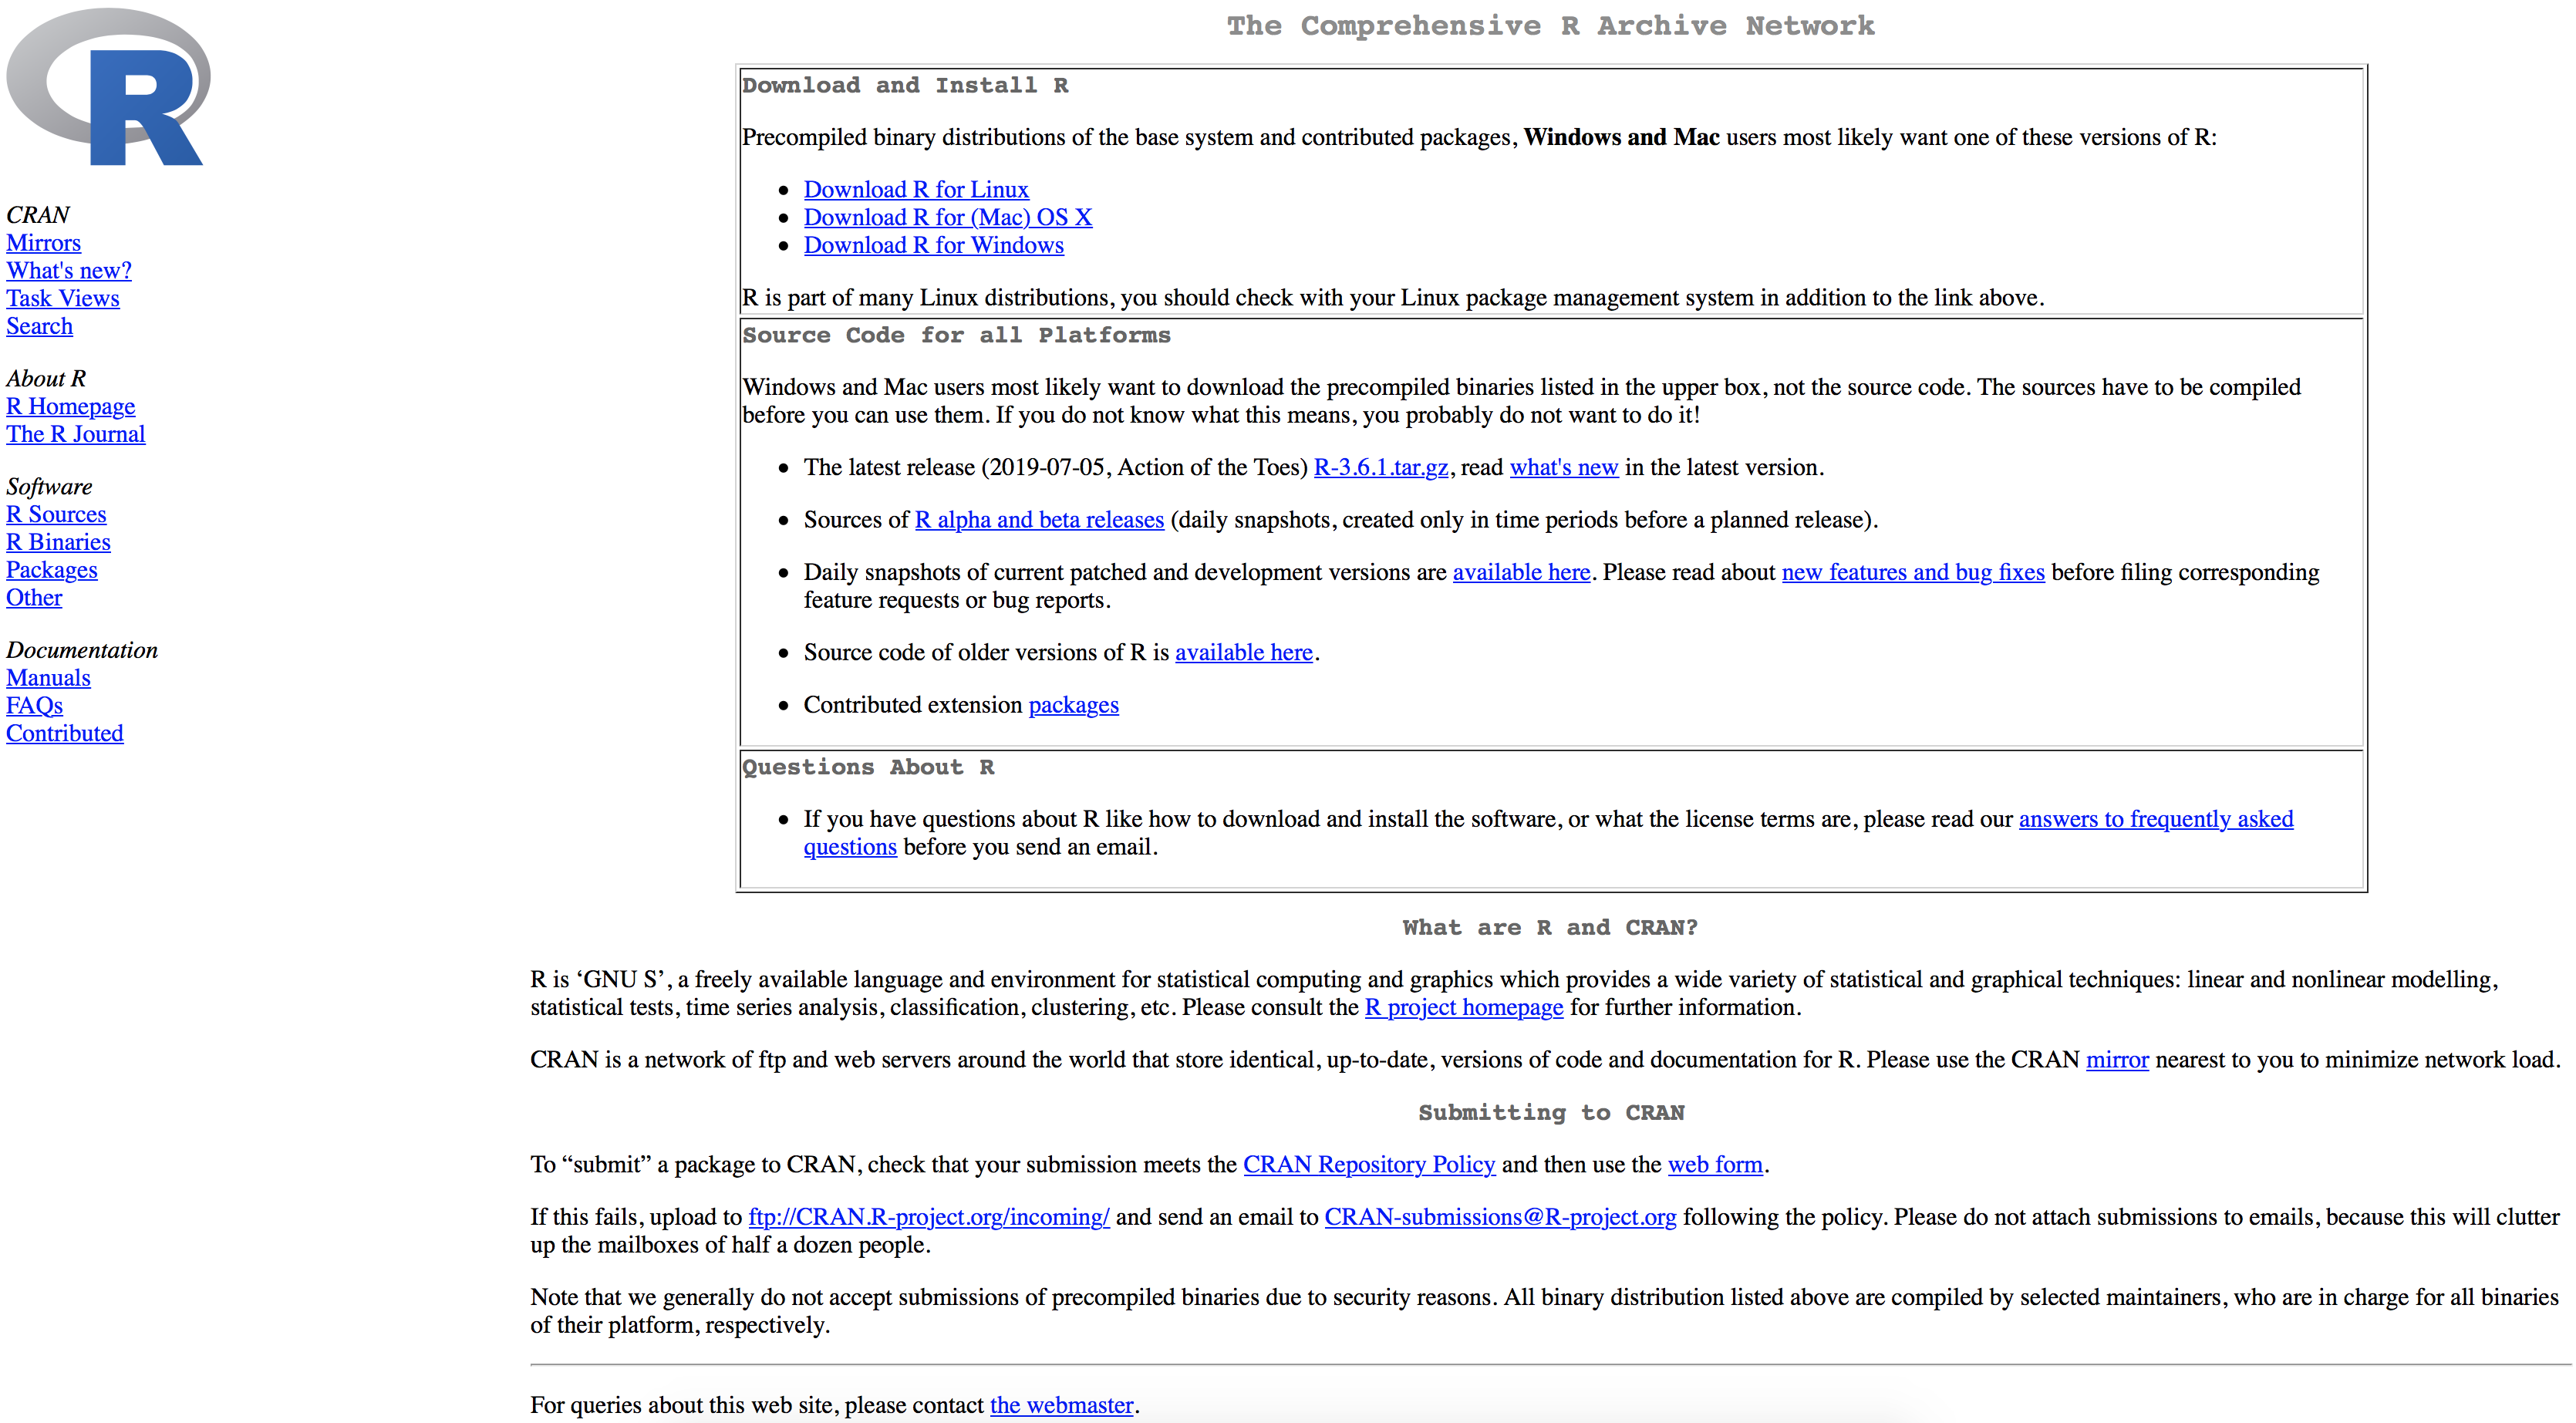
\includegraphics[width=0.9\linewidth]{figures/ch3_cran}
%\caption{The Comprehensive R Archive Network.}
%\label{fig:cran}
%\end{figure}

After installing R, let's immediately install RStudio Desktop (the free version).
Go to \url{https://rstudio.com/products/rstudio/download/#download} and download and run the installer for your computer.
If you open RStudio you should get a screen similar to \reffig{rstudio}.
If this is the first time you open RStudio you probably don't see the top left pane (the scripts),
you can create that pane by creating a new \emph{R Script} via the \emph{file} menu or with the green plus icon in the top left corner. 

\begin{figure}
\centering
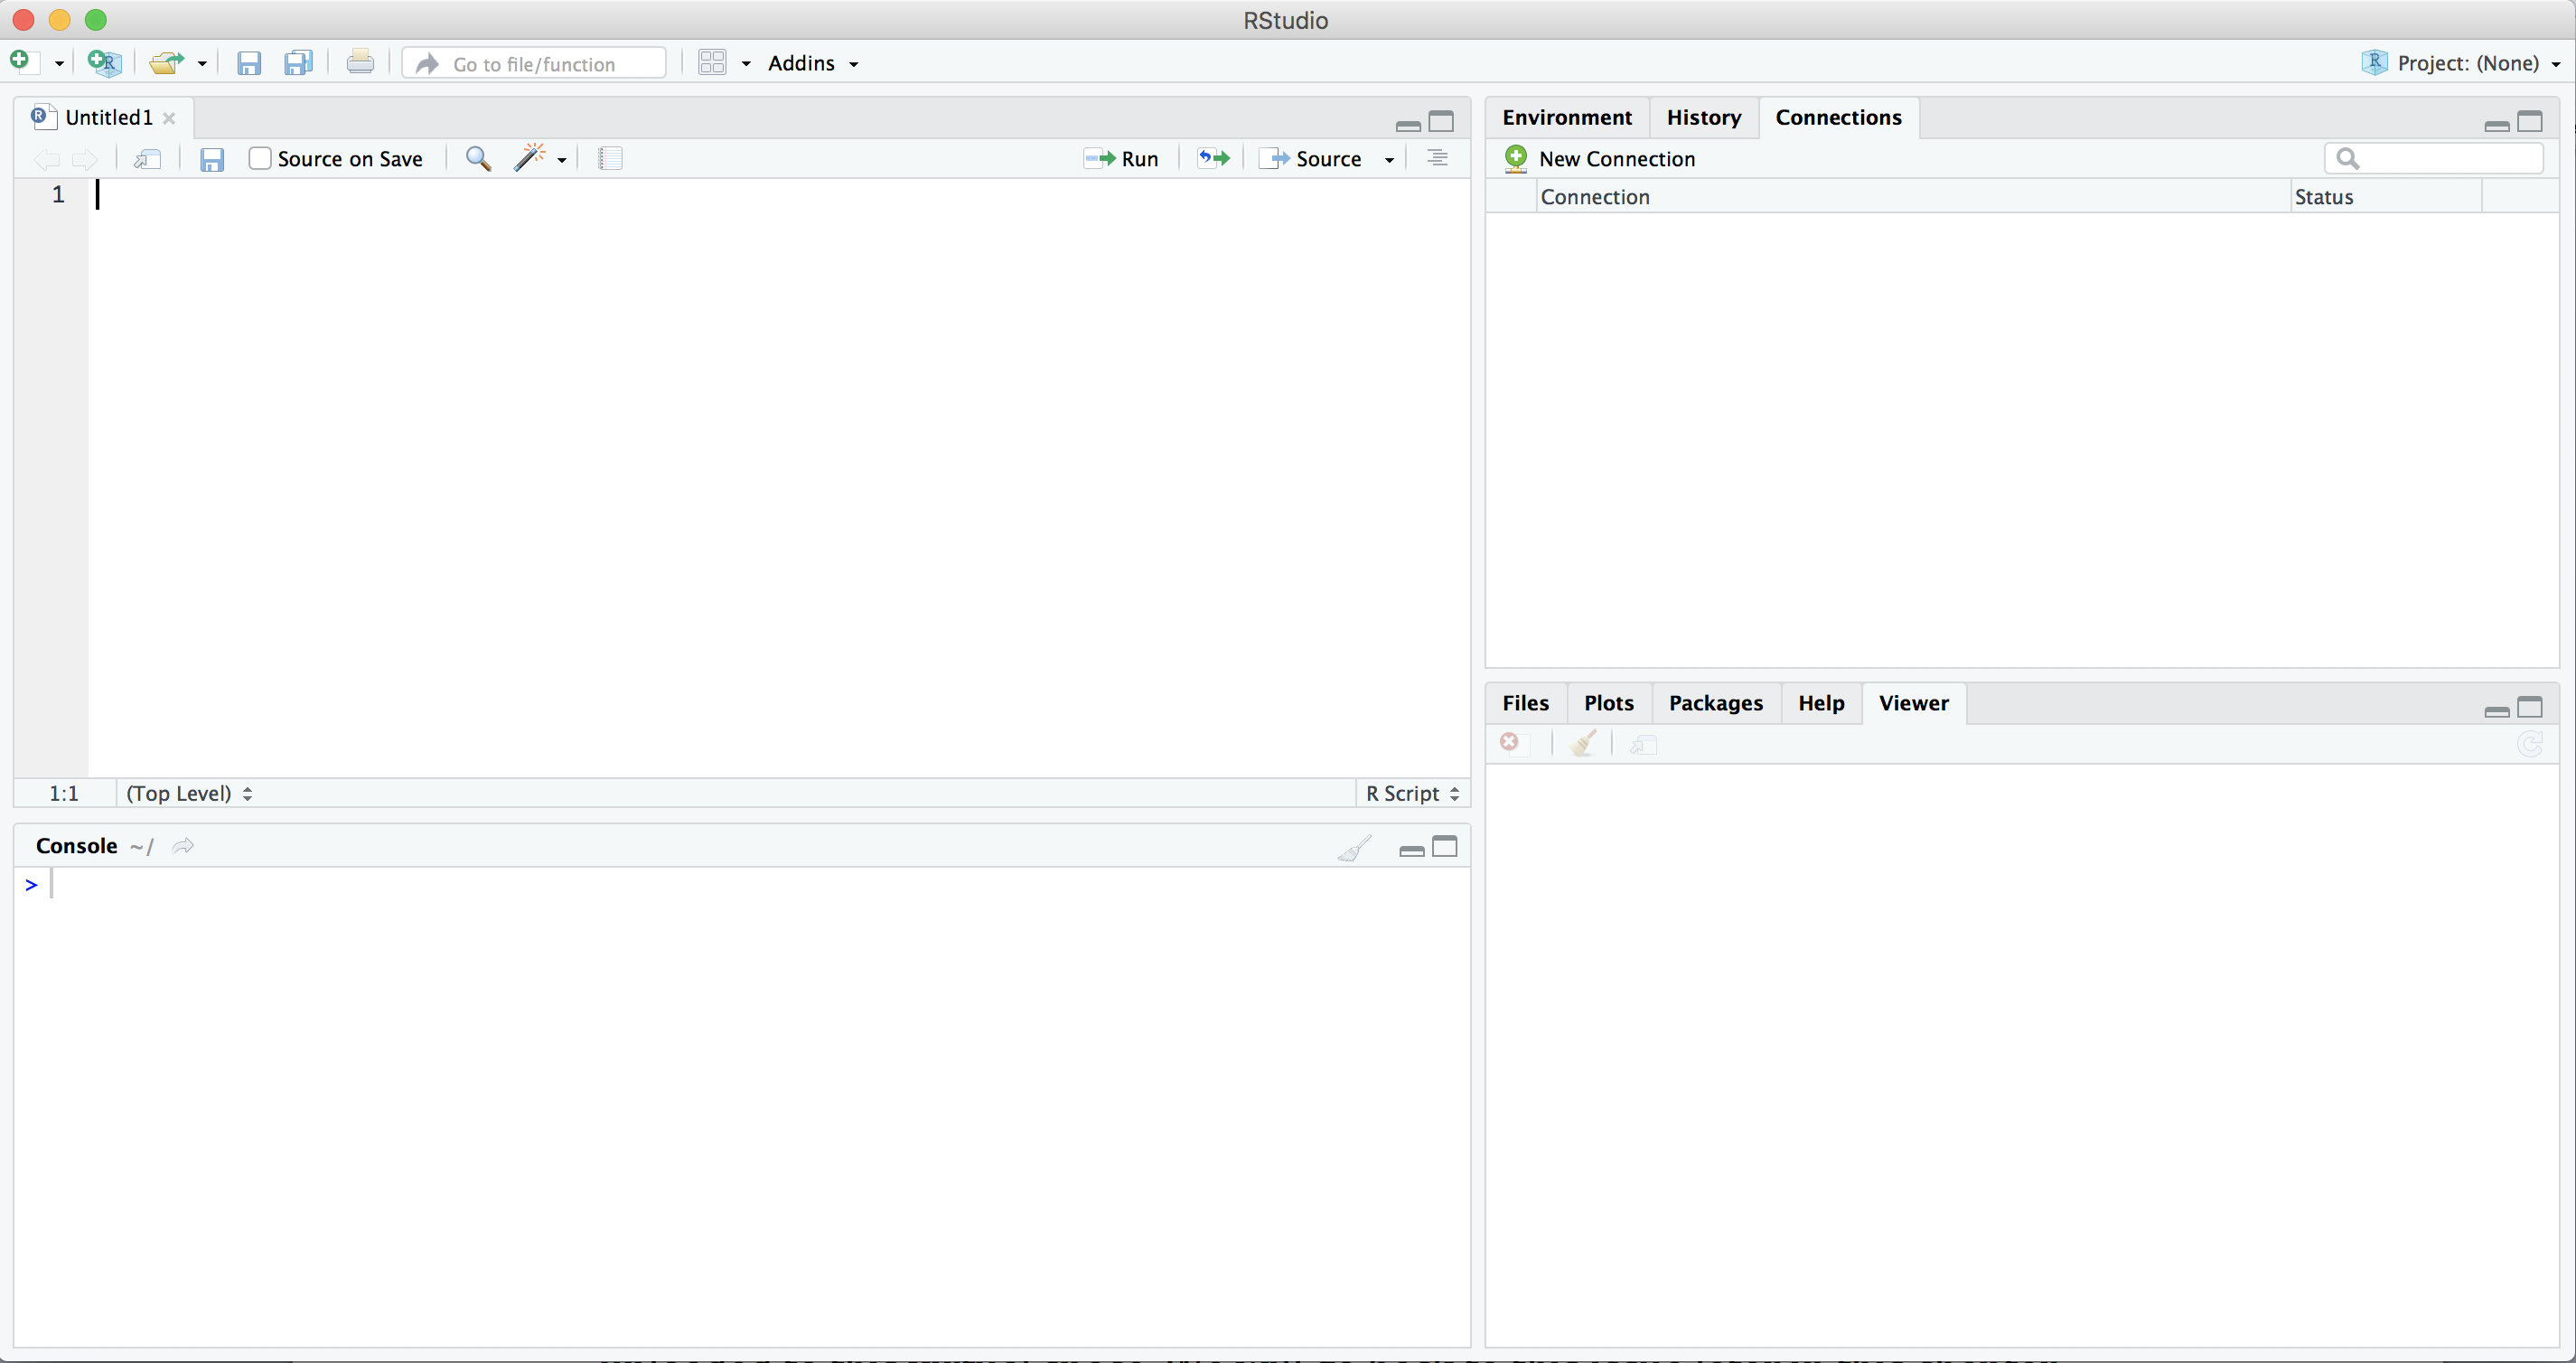
\includegraphics[width=0.9\linewidth]{figures/ch3_r_studio}
\caption{RStudio Desktop}
\label{fig:rstudio}
\end{figure}

Of the four panes in RStudio,
you will probably spend most time in the top left pane, where you can view and edit your analysis \emph{scripts}.
A script is simply a list of commands that the computer should execute one after the other,
for example to open your data, do some computations, and make a nice graph. 

To run a line of code, you can place your cursor anywhere on that line and click the \emph{Run} icon or
press control+Enter.
To try that, type the following into your newly opened script:

\verb|print("Hello world")|

Now, place your cursor on that line and press Run (or control+Enter).
What happens is that the line is copied to the \emph{Console} in the bottom left corner
and executed.
So, the results of your commands (and any error messages) will be shown in this console view

Contrary to most traditional programming languages,
the easiest way to run R code is line by line.
You can simply place your cursor on the first line,
and repeatedly press control+Enter, which executes a line and then places the cursor on the next line.
You can also select multiple lines (or part of a line) to execute those commands together,
but in general it is easiest to check that everything goes as planned if you run the code line by line.

You can also write commands directly in the console and execute them (by pressing enter).
This can be useful for trying things out or to run things that only need to be run once,
but in general we would strongly recommend typing all your commands in a script and then executing them.
That way, the script serves as a log of what commands you have run to analyse your data,
so you (or a colleague) can read and understand how you did the analyses. 

\begin{feature}
  \textbf{RStudio Projects}
  A very good idea to organize your data and code is to work with RStudio Projects.
  In fact, we would recommend you to now create a new empty project for the examples in this book.
  To do this, click on the \emph{Project} button in the top right and select `New Project'.
  Then, select New Directory and New Project and enter a name for this project
  and a a parent folder for the project if you don't want it in your Documents. 
  Using a project means that the scripts and data files for your project are all in the same location
  and you don't need to mess around with specifying the locations of files
  (which will probably be different for someone else or on a different computer).
  Morever, RStudio remembers which files you were editing for each project,
  so if you are working on multiple project it's very easy to switch between them.
  We recommend creating a project now for the book (and/or for any projects you are working on),
  and always switching to a project when you open RStudio
\end{feature}


On the right side of RStudio workspace you will find two additional
windows. In the top right pane there are two or more tabs:
\emph{environment} and \emph{history}, and depending on additional
packages you may have installed maybe some more.  In
\emph{environment} you can manage your workspace (the set of elements
you need to deploy for data analysis) and have a list of the objects
you have uploaded to it. You may also import datasets with this tool.
In the \emph{history} tab you
have an inventory of code executions, which you can save to a file, or
move directly to console or to an R document.

Note that in the environment you can save and load your ``workspace'' (all data in the computer memory).
However, relying on this functionality is often not a good idea: it
will only save the state of your current session, whereas you most
likely want to save your R syntax file and/or your data instead.
If you have your raw input data (e.g., as a csv file, see \refchap{filetodata})
and your analysis script, you can always
reproduce what you have been doing. If you only have a snapshot of
your workspace, you know state in which you arrived, but cannot
necessarily reproduce (or change) how you got there.

In the bottom right pane there are five additional useful tabs.
In \emph{files} you can explore
your computer and manage all the files you may use for the project,
including importing datasets. In \emph{plots}, \emph{help} and
\emph{viewer}, you can visualize the outputs figures, documentation
and general outcomes, respectively, that you have executed in your
script. Finally, the tab for \emph{packages} will be of great
utility since it will let you install or update packages from CRAN or
even from a file saved on your computer with a friendly interface.

\subsection{Installing Python and Jupyter Notebook}

Python is an object-orientated programming language
and it is probably the favourite language of computational and data
scientists in all disciplines around the world.
There are different releases of Python, but the biggest difference used to be between Python 2 and Python 3.
Fortunately, you will probably never need to install or use Python 2, and in fact it is no longer supported since January 2020.
Thus, you can just use any recent Python 3 version for this book.
When browsing through questions on online fora such as Stackoverflow or reading other people's code on Github (we will talk about that in \refchap{worldcode}), you still may come across legacy code in Python 2. Such code usually does not run directly in a Python 3 interpreter, but in most cases, only minor adaptions are necessary to make it work.

We will install and run Python and Jupyter Notebook using a \concept{terminal} or command line interface.
This is a tool that is installed on all computers that allows you to give commands to the computer directly.
First, create a project folder for this book using the File Explorer / Finder.
Then, on Windows you can shift + Right click that folder and select ``Open command Window here''.
On MacOS, after navigating to the folder you just created, you click on ``Finder'' in the menu at the top of the screen, then on ``Services'', then on ``New Terminal at Folder''
In both cases, this should open a new window (usually black or grey) that allows you to type commands.

Note that on most computers, Python is already installed by default.
%Note that on many computers, especially on MacOS and Ubuntu, python is already installed by default.
You can check this by typing the following the command in your terminal:

\begin{verbatim}
python3 --version
\end{verbatim}

On some versions of Windows, you may need to use \verb|py| instead of \verb|python3|:
\begin{verbatim}
py --version
\end{verbatim}

In either case, the output of this command should be something like \verb|Python 3.8.5|.
If \verb|python --version| also returns this version, you are free to use either command
(but on older systems \verb|python| can still refer to Python 2, so make sure that you are using Python 3 for this book!).

If Python is not installed on your system, go to \url{https://www.python.org/downloads/windows/} or \url{https://www.python.org/downloads/mac-osx/} and download and install the latest stable release (which at the time of writing is \verb|3.9.0|).
\footnote{For linux, install python3 and pip using your package manager. For example, on ubuntu you can run \texttt{sudo apt install python3-pip}}
After installing it, open a terminal again and run the command above to verify that it is installed correctly.

Included in any recent Python install is \concept{pip}, the program that you will use for installing python packages.
You can check that pip is installed correctly by typing the following command on your terminal:

\begin{verbatim}
pip3 --version
\end{verbatim}

Which should report something like \texttt{pip 20.0.2 from ... (python 3.8)}.
Again, if \verb|pip| reports the same version you can also use it instead of pip3.
On some systems \verb|pip3| will not work, so use \verb|pip| in that case
(but make sure to check that it points to Python 3).

\paragraph{Installing Jupyter Notebook}
Next, we will install Jupyter Notebook, which you can use to run all the examples in this book
and is a great environment for developing python data analysis scripts.
Jupyer Notebooks (which are also included in IDE JupyterLab if you installed that), 
are run as a web application
that allows you to create documents that contain code and inline text fragments.
 One of the nicest things of
the Jupyter Notebook is that the code is inserted in fields (so-called ``cells'') that you
can run one by one, getting its respective output, which added to the
designed narrative text will make your script more clean and
reproducible. You can also add formatted text blocks (using a simple formatting language called \concept{Markdown})
to explain to the reader what you are doing. In \refsec{practices}, we will address
notebooks again as a good practice for a computational scientist.

You can install jupyter notebook directly using pip using the following command
(executed in a terminal):

\begin{verbatim}
pip3 install jupyter-notebook
\end{verbatim}

Now, you can run jupyter by executing the following command on the terminal:

\begin{verbatim}
jupyter notebook
\end{verbatim}

This will print some useful information, including the URL at which you can access the notebook.
However, it should also directly open this in a browser (e.g. Chrome) so you can directly start working. 
In your browser you should see a juypter screen similar to the middle window in \reffig{jupyter}.
Create a new notebook by clicking on the \emph{New} button in the top right and selecting Python 3.
This should open a window similar to the bottom window in \reffig{jupyter}.

\begin{figure}
  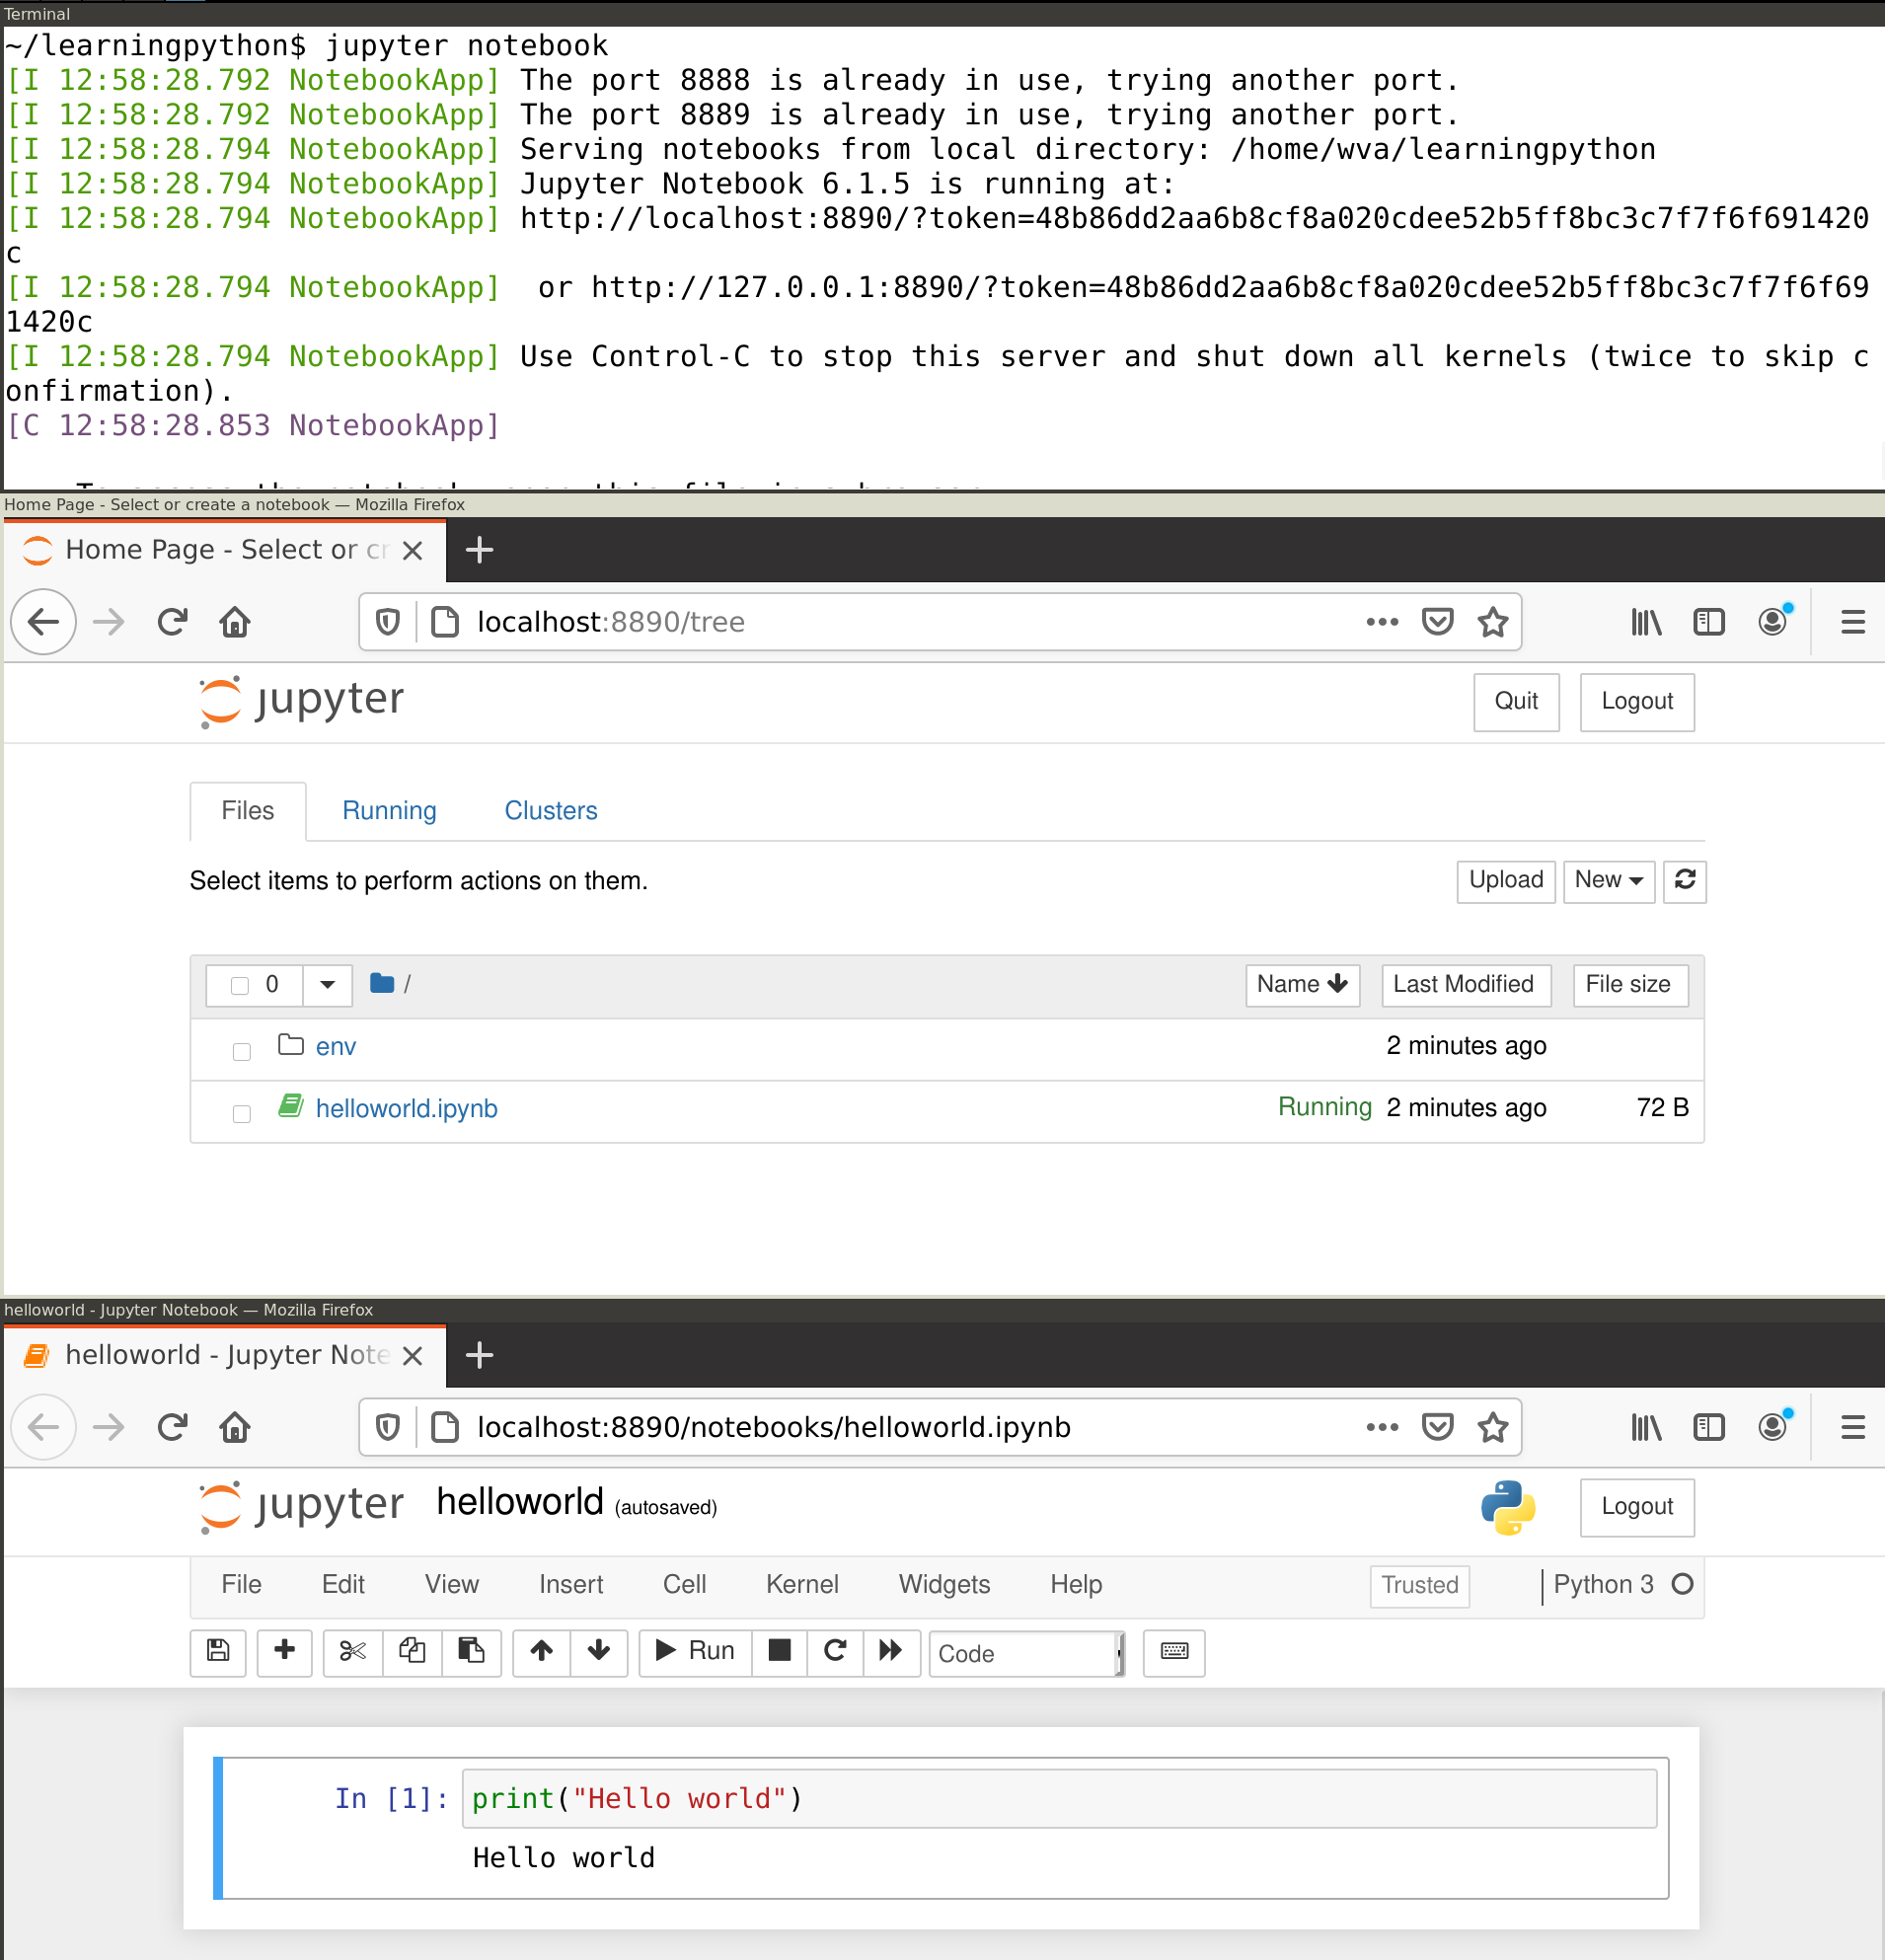
\includegraphics[width=\textwidth]{figures/jupyter.png}
  \caption{Jupyter Notebook}\label{fig:jupyter}
\end{figure}

In jupyter, code is entered into cells.
First, type \verb|print("Hello World")| into the empty cell next to the \verb|In [ ]:| prompt.
Then, click the Run button or press control+Enter. This should execute your command and display
the text \verb|"Hello World"| in the output area right below the input cell.
Note that you can create more cells using the plus icon or with the insert menu.
You can also set the cell type via the Cell menu: select code for analysis scripts (which is the default),
or Markdown for text fragments, which can be used to explain the code and/or interpret the results.

\section{Installing third-party packages}

The \fn{print} function used above is included automatically when you start R or Python.
Many functions, however, are included in separate \concept{packages} (also known as \concepts{libraries} or \concept{modules}), which are
generally collections of commands for a certain task or activity.

Although both R and Python come pre-installed with many useful \concept{packages},
one of the great things of both languages is that they have a very active community that continuously develops, improves, and publishes new packages.
Throughout this book, we will be using such third-party packages for a variety of tasks, from data wrangling and visualization to text analysis.
For example, we will use the R package \pkg{tidyverse} and the Python packages \pkg{pandas} for data wrangling.

To install these packages on your computer, run the following commands:
(Note: if you are using Anaconda, replace \ttt{pip3 install} by \ttt{conda install})  

\begin{tcbraster}[raster columns=2,raster equal height=rows,raster valign=top]
   \codex[caption=Installing a package from Jupyer]{chapter01/ch01install.py}
   \codex[caption=Installing a package in R]{chapter01/ch01install.r}
\end{tcbraster}

\newcommand{\fnrepo}{\footnote{Similar to the App Store or Play Store, both R and Python have a centralized repository for third party packages.  For R, this is the Comprehensive R Archive Network (CRAN) encountered earlier,
    while for Python this is the Python Package Index (PyPI) accessed by \verb|pip|.  Normally, all packages in these repositories are open source and safe to install.}}

These commands will automatically fetch the package from the right repository\fnrepo and install them on your computer. This can take a while, especially for large packages such as tidyverse.
Fortunately, this only needs to be done once.
Every time time you use a package, you also need to \emph{activate} it using the \fn{import} (Python) or  \fn{library} (R) command.

In general, whenever you get an error \texttt{No module named 'pandas'} (Python) or \texttt{there is no package called ‘tidyverse’},
you can just install the package with that name using the code listed above.
If you get an error such as \texttt{name 'pandas' is not defined} (Python) or \texttt{object 'ggplot' not found} (R),
it is quite possible you forgot to activate the package that includes that function. 


\begin{feature}
\textbf{Packages used in each chapter}\\
Some packages, like the \pkg{tidyverse} (R) and \pkg{pandas} (Python) packages for data handling are used in almost every chapter.
Many chapters also introduce specific packages such as \pkg{igraph}/\pkg{networkx} for network analysis in \refchap{network}.
To make it easy to keep track of the packages needed for each chapter,
every chapter that includes code in this book starts with a note like this that gives an overview of the main packages introduced in that chapter.
It also includes the code needed to install these packages, which of course is only needed if you didn't install these packages before.
Note again that if you are using Anaconda for Python,
your should replace \ttt{!pip3 install} by \ttt{!conda install} in that code. On some systems, you may need to use \ttt{!pip install} instead of \ttt{!pip3 install}.

These note also includes a code block to import all the packages used for that chapter,
which you need to run every time you use examples from that chapter.
\end{feature}
